\section{Results}
\label{sec:results}
\emph{Note that measurements for the Generalized RRR with arity 16 are missing, since the experiments took too long due to paging.}

\emph{Also Note that the Uncompressed Wavelet Tree timings have been plotted on 
a different graph due to the difference in scale.}\\

From Figure \ref{fig:stime-eng}, we can see how increasing the arity affects
querying a non-compressed Wavelet Tree. It is slower for increasing file size
because it is calculating rank queries without the assistance of RRR.


		\DefFig[English]
			{fig:stime-eng}{experiments/simple_time_english}{0.9}
			{Query times for Uncompressed Multiary Wavelet Tree of increasing 
			arity for each \emph{English} file.}
		
			\begin{figure}[h]
			\begin{center}$
			\begin{array}{cc}
			\mbox{English (25MB)} & \mbox{English (50MB)} \\
			\includegraphics[width=2.5in]{experiments/time_english_25MB} &
			\includegraphics[width=2.5in]{experiments/time_english_50MB}
			\end{array}$
			\end{center}
			\caption{Query times for RRR Wavelet Trees of increasing arity
			for the 25MB and 50MB \emph{English} files.}
			\label{fig:time-eng-25-50}
			\end{figure}
		
		\DefFig[English (75MB)]
			{fig:time-eng-75}{experiments/time_english_75MB}{0.9}
			{Query times for RRR Wavelet Trees of increasing arity
			for the 75MB \emph{English} file.}

From Figures \ref{fig:time-eng-25-50} and \ref{fig:time-eng-75} we are able 
to see that increasing the file size does not significantly affect the time
performance of the Wavelet Trees which utilise RRR.

The Generalised RRR is slower than Claude's. We suspect that this is due to our 
use of pointers required to create a sparse table, whereas Claude's avoids 
dereferencing and makes better use of cache. The trend is similar to the
other multiary Wavelet Trees, though. the `Multi-Binary RRR' Wavelet Tree
is faster than Claude's when the arity is increased, but appears to plateau.

All other time graphs show similar trends, and so have been omitted\footnote{The 
other graphs are available at http://github.com/alexbowe/honours-thesis/}.

		\DefFig[Words (75MB)]
			{fig:mem-eng-75}{experiments/mem_english_ints_75MB}{0.9}
			{Memory consumption for Wavelet Trees of increasing arity for
			the 75MB \emph{Words} file. The size coefficient is a multiplier
			on the original file size. The bar stacked on top is the space for
			the supporting RRR table. The bar underneath is the space for
			the Wavelet Tree (which had negligible overhead) and each of its
			nodes, as RRR sequences or not. The Uncompressed Wavelet Tree is
			the only one which does not have a RRR table.}

Figure \ref{fig:mem-eng-75} shows how changing the arity affects the memory
consumption of the structures. We only show this for the 75MB file, as the 
others compress (or expand) with similar coefficients. Note that even though 
the generalised RRR structure's Wavelet Tree (which includes the RRR sequences 
it stores) is smaller than the original text, the size to contain the supporting 
RRR count structure is very large.

		\DefFig[Proteins (75MB)]
			{fig:mem-prot-75}{experiments/mem_proteins_75MB}{0.9}
			{Memory consumption for Wavelet Trees of increasing arity for
			the 75MB \emph{Proteins} file. The size coefficient is a multiplier
			on the original file size. The bar stacked on top is the space for
			the supporting RRR table. The bar underneath is the space for
			the Wavelet Tree (which had negligible overhead) and each of its
			nodes, as RRR sequences or not. The Uncompressed Wavelet Tree is
			the only one which does not have a RRR table.}


\begin{figure}[h]
\begin{center}$
\begin{array}{cc}
\mbox{English} & \mbox{Words} \\
\includegraphics[width=2.5in]{experiments/unique_english} &
\includegraphics[width=2.5in]{experiments/unique_english_ints} \\ \\ \\
\mbox{DNA} & \mbox{Proteins} \\ 
\includegraphics[width=2.5in]{experiments/unique_dna} &
\includegraphics[width=2.5in]{experiments/unique_proteins} \\ \\ \\
\mbox{Sources} & \mbox{XML} \\
\includegraphics[width=2.5in]{experiments/unique_sources} &
\includegraphics[width=2.5in]{experiments/unique_dblp_xml}
\end{array}$
\end{center}
\caption{Number of unique values of each class and permutation for each data 
file. The Y axis represents the total number of classes or 
permutations that were witnessed for the given file size and arity when using 
the Multiary Wavelet Tree with Generalised RRR.}
\label{fig:unique}
\end{figure}
	
\begin{figure}[h]
\begin{center}$
\begin{array}{cc}
\mbox{English} & \mbox{Words} \\
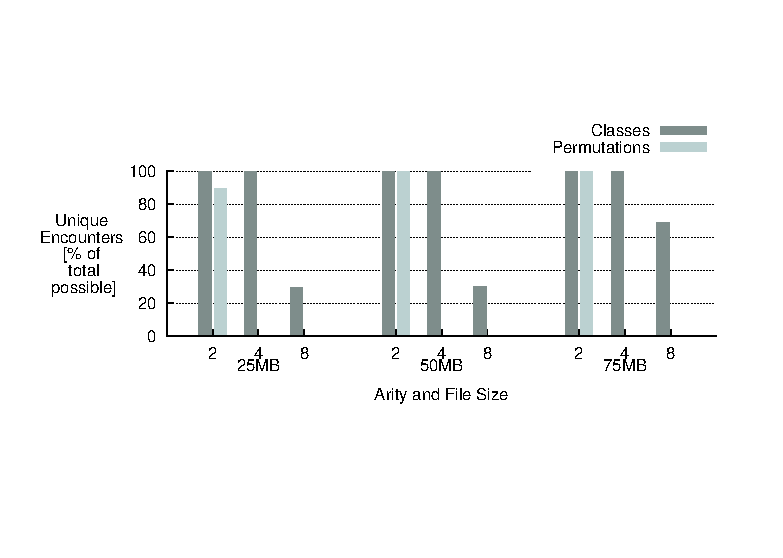
\includegraphics[width=2.5in]{experiments/sparse_english} &
\includegraphics[width=2.5in]{experiments/sparse_english_ints} \\ \\ \\
\mbox{DNA} & \mbox{Proteins} \\ 
\includegraphics[width=2.5in]{experiments/sparse_dna} &
\includegraphics[width=2.5in]{experiments/sparse_proteins} \\ \\ \\
\mbox{Sources} & \mbox{XML} \\
\includegraphics[width=2.5in]{experiments/sparse_sources} &
\includegraphics[width=2.5in]{experiments/sparse_dblp_xml}
\end{array}$
\end{center}
\caption{Sparsity measurements for each data file. The Y axis represents
the percentage of \emph{total possible} classes or permutations that were
witnessed for the given file size and arity when using the 
Multiary Wavelet Tree with Generalised RRR.}
\label{fig:sparse}
\end{figure}

The large size of the RRR Table for the Generalised RRR in Figure 
\ref{fig:mem-prot-75} appears to be the result of the large number of unique
permutations encountered for the Proteins file, since it has less classes but 
more permutations than the words file. See Tables .. and \ref{tab:maxclass}.

\begin{table}[h]
\begin{center}
\begin{tabular}{crr}
\toprule
Arity & \multicolumn{1}{c}{Max Total Classes} &
\multicolumn{1}{c}{Max Total Permutations}\\
\midrule
2 & 16 & 32 768\\
4 & 816 & 1 073 741 824\\
8 & 17 0544 & 35 184 372 088 832\\
\bottomrule
\end{tabular}
\caption{Maximum Total Classes and Offsets possible with a blocksize of 15 for arity 
    values 2, 4, and 8.}
\label{tab:maxclass}
\end{center}
\end{table}

